\documentclass[nobib]{tufte-handout}

\title{Lecture 3: Common graph families, trees, and Cayley's theorem $\cdot$ 1MA020}

\author[Vilhelm Agdur]{Vilhelm Agdur\thanks{\href{mailto:vilhelm.agdur@math.uu.se}{\nolinkurl{vilhelm.agdur@math.uu.se}}}}

\date{24 October 2023}


%\geometry{showframe} % display margins for debugging page layout

\usepackage{graphicx} % allow embedded images
  \setkeys{Gin}{width=\linewidth,totalheight=\textheight,keepaspectratio}
  \graphicspath{{graphics/}} % set of paths to search for images
\usepackage{amsmath}  % extended mathematics
\usepackage{booktabs} % book-quality tables
\usepackage{units}    % non-stacked fractions and better unit spacing
\usepackage{multicol} % multiple column layout facilities
\usepackage{lipsum}   % filler text
\usepackage{fancyvrb} % extended verbatim environments
  \fvset{fontsize=\normalsize}% default font size for fancy-verbatim environments

\usepackage{color,soul} % Highlights for text

% Standardize command font styles and environments
\newcommand{\doccmd}[1]{\texttt{\textbackslash#1}}% command name -- adds backslash automatically
\newcommand{\docopt}[1]{\ensuremath{\langle}\textrm{\textit{#1}}\ensuremath{\rangle}}% optional command argument
\newcommand{\docarg}[1]{\textrm{\textit{#1}}}% (required) command argument
\newcommand{\docenv}[1]{\textsf{#1}}% environment name
\newcommand{\docpkg}[1]{\texttt{#1}}% package name
\newcommand{\doccls}[1]{\texttt{#1}}% document class name
\newcommand{\docclsopt}[1]{\texttt{#1}}% document class option name
\newenvironment{docspec}{\begin{quote}\noindent}{\end{quote}}% command specification environment

\include{mathcommands.extratex}

\begin{document}

\maketitle% this prints the handout title, author, and date

\begin{abstract}
\noindent
We start by introducing a few named families of graphs. Then we introduce the class of \emph{trees}, and prove some results about them, such as that they have leaves.\sidenote[][]{Contradicting what our own eyes can see outside in the November weather.} The main result is Cayley's theorem, which counts the number of labelled trees on $n$ vertices.
\end{abstract}

\section{Common graph families}

We warm up today by giving names to some common families of simple graphs that we will see reappearing throughout the course. They are illustrated in Figure \ref{fig:graph_families}.

\begin{figure}
  \centering
  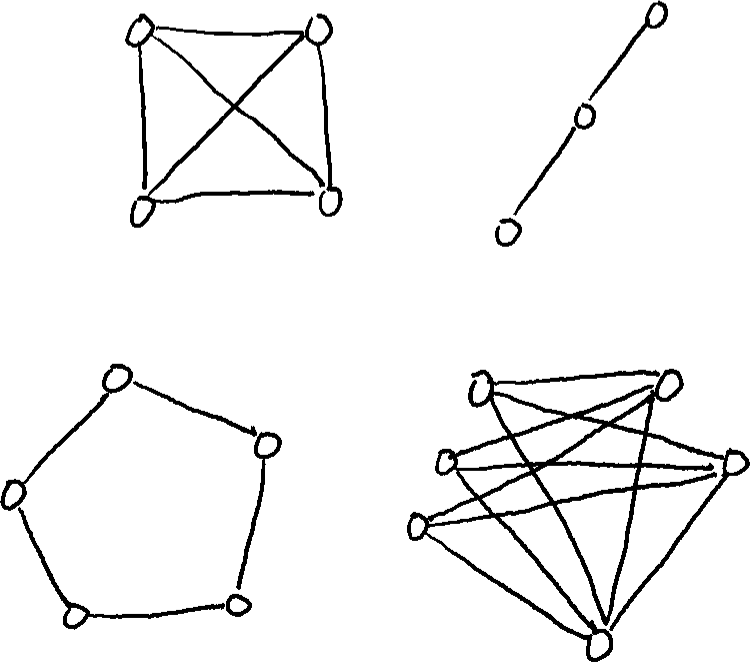
\includegraphics[width=0.5\textwidth]{graphics/L3_trees/graph_families.png}
  \caption[][0cm]{Four graphs: $K_4$, $P_2$, $C_5$, and $K_{3,2,1}$.}
  \label{fig:graph_families}
\end{figure}

\begin{enumerate}
  \item The complete graphs on $n$ vertices, denoted $K_n$. These contain all the $\binom{n}{2}$ potential edges. These are also called \emph{cliques} when we see them as subgraphs of a bigger graph.
  \item The paths of length $\ell$, denoted $P_\ell$. If we take the set $\{0,1,\ldots,\ell\}$ to be our vertex set, the edges are precisely of the form $\{i-1,i\}$ for $i \in [\ell]$.\sidenote[][]{This is another notation you might not have seen before: For an integer $n$, we write $[n]$ for the set $\{1, 2, \ldots, n\}$}
  \item The cycle graphs on $n$ vertices, denoted $C_n$. We can think of these as a path of length $n-1$ with an extra edge joining the first and last vertex.
  \item The complete bipartite graphs on $a + b$ vertices, denoted $K_{a,b}$. These have as vertex set the disjoint union of two sets $L$ and $R$,\sidenote[][]{Think of these as the ``left'' and ``right'' vertices.} with $\abs{L} = a$ and $\abs{R} = b$, and there is an edge between $v$ and $w$ whenever $v \in L$ and $w \in R$. When we see these graphs as subgraphs of a bigger graph, we sometimes also call them \emph{bicliques}.
  \item Generalizing the complete bipartite graphs, the complete multipartite graph on $r$ parts with sizes $a_1, a_2, \ldots a_r$, denoted $K_{a_1, a_2, \ldots, a_r}$, has as its vertex set the disjoint union of $r$ sets $V_1, V_2, \ldots, V_r$, where $\abs{V_i} = a_i$, and there is an edge between two vertices whenever they are not in the same part. We can notice that when $r=2$ this is a complete bipartite graph, and when all the parts are of size $1$ this is a complete graph.
\end{enumerate}

For most of these, it is obvious how many edges they will have. Let us state a lemma that shows how many the complete multipartite graphs have.

\begin{lemma}
  The complete multipartite graph $K_{a_1, a_2, \ldots, a_r}$ has $\frac{1}{2}\left(n^2 - a_1^2 - \ldots - a_r^2\right)$ edges.

  \begin{proof}
    We use the handshake lemma from the previous lecture. Since a vertex in $V_i$ has one edge to every vertex not in $V_i$, it has degree $n - a_i$, and there are $a_i$ such vertices. Thus we can compute that
    \begin{align*}
      2\abs{E} &= \sum_{v\in V} d_v
      = \sum_{i=1}^r \sum_{v \in V_i} d_v\\
      &= \sum_{i=1}^{r} \sum_{v \in V_i} (n - a_i)
      = \sum_{i=1}^{r} a_i(n - a_i)\\
      &= n\left(\sum_{i=1}^{r} a_i\right) - \sum_{i=1}^{r} a_i^2
      = n^2 - \sum_{i=1}^{r} a_i^2
    \end{align*}
    proving the claim.
  \end{proof}
\end{lemma}

\begin{corollary}
  The complete bipartite graph $K_{a,b}$ has $\frac{1}{2}\left(n^2 - a^2 - b^2\right) = ab$ edges.
\end{corollary}

\section{Trees}

The main topic of this lecture is the so-called \emph{trees}. Informally, they are just graphs that look like trees -- though with this intuition we are drawing them upside-down.\sidenote[][]{Unless you are a computer scientist, in which case you draw them the right way up, I believe.}

\begin{definition}
  A \emph{tree} is a graph $T = (V,E)$ that is both connected and contains no cycles.
\end{definition}

Just like for graphs in general, there are countless variants of the notion of a tree. We can give the tree a root,\sidenote[][]{Which is quite necessary for a biological tree.} we can consider orderings of the vertices in various ways, and so on. None of this will actually be necessary in the course, however, so we skip defining these notions.

\begin{example}
  Trees appear in many places in various areas -- one common place for them to appear is in the study of algorithms. Let's study the quicksort algorithm, and see how it can be represented as a tree. The algorithm sorts a list of numbers in ascending order, and it works as follows:
  \begin{enumerate}
    \item Fix an arbitrary pivot $p$ element from the list.
    \item Compare all non-pivot elements with the pivot, and put the ones that are smaller in a list we call $L$, and the ones that are larger in a list we call $R$.\sidenote[][-1.8cm]{This is of course not the most efficient way to \emph{implement} this algorithm -- the correct thing to do is to move elements around in a single list, since this can be done ``in place'' and so will be faster. But this is mathematically equivalent, and easier to phrase.}
    \item Apply the quicksort algorithm to $L$ and $R$ if they contain more than one element.\sidenote[][-0.3cm]{Since we did not include the pivot element in either set, they are both strictly shorter lists than the one we started with, so this recursion will terminate.}
    \item Return the list $LpR$.
  \end{enumerate}

  We can represent this algorithm with a rooted ordered binary\sidenote[][]{Binary in the sense of a computer scientist, since this is after all an algorithm. A mathematician would have a slightly different definition of binary tree.} tree. This means the tree has one designated vertex we call the root, and every vertex has potentially a left child and a right child, where a ``child'' is a neighbour who is further from the root than themselves.

  We create a tree from this algorithm by letting the pivot element be the root of the tree, and then recursively letting its left child be the root of of the tree quicksort gives us for the list $L$, and the right child be the root of the tree we get for the list $R$. This hopefully becomes clearer if we work through an example:

  Consider the list $3,7,1,4,9,8,6,2,5$, and choose $7$ as our pivot element. Then we get $L = 3,1,4,6,2,5$ and $R = 9,8$.

  So, recursing, we now need to sort the list $3,1,4,6,2,5$, and we pick $3$ as our pivot element, getting a new $L = 1,2$ and $R = 4,6,5$. If we pick $1$ as our pivot in $L$, we get $L = \emptyset$ and $R = 2$. Picking $5$ as out pivot in the previous $R$, we get $L = 4$ and $R = 6$.

  \begin{figure}
    \centering
    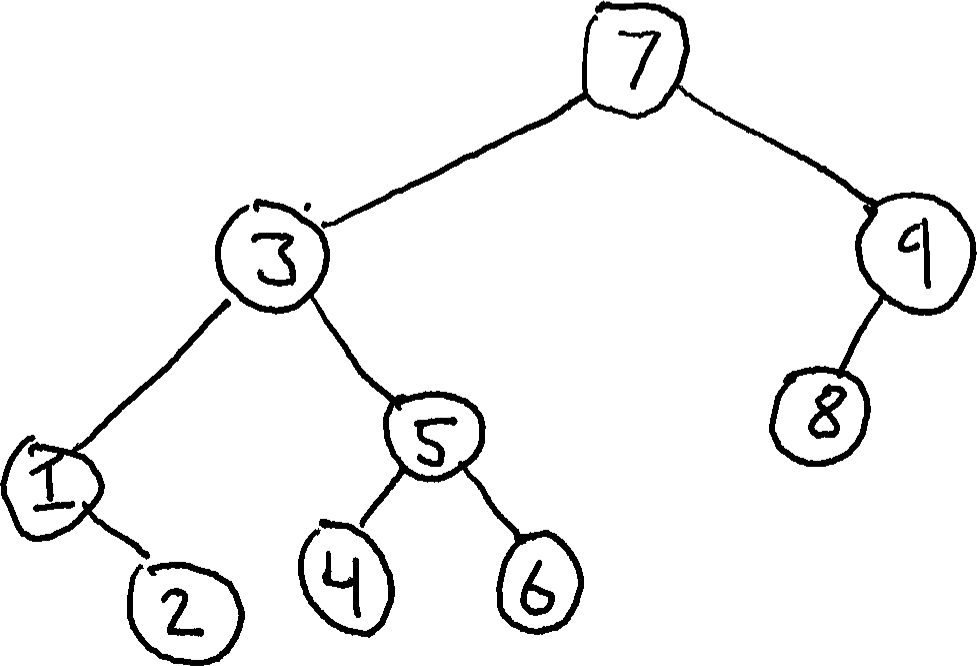
\includegraphics[width=0.6\textwidth]{graphics/L3_trees/quicksort_tree.png}
    \caption[][0cm]{A tree gotten from quicksorting a list of integers in our example.}
    \label{fig:quicksort_tree}
  \end{figure}

  Finally, we need to quicksort the list $9,8$, where we can pick $9$ as our pivot and get $L = 8$, $R = \emptyset$. The resulting tree of what we just did is drawn in Figure \ref{fig:quicksort_tree}.
\end{example}

Having seen this example of a place where trees appear, let us start proving some properties of trees.

\begin{lemma}\label{lemma:trees_have_leaves}
  Every finite\sidenote[][]{
    \begin{xca}
      Why do we need the finiteness assumption?
    \end{xca}
  } tree with at least $2$ vertices contains at least two vertices of degree $1$. Such vertices are called leaves.

  \begin{proof}
    Let $T$ be a finite tree on at least two vertices. Consider a path $P = x e_1 x_1 e_2 \ldots y$ of maximum length in $T$. Assume for contradiction that one of $x$ and $y$ -- w.l.o.g.,\sidenote[][]{``without loss of generality''.} let's say $x$ -- has degree at least $2$.

    \begin{figure}
      \centering
      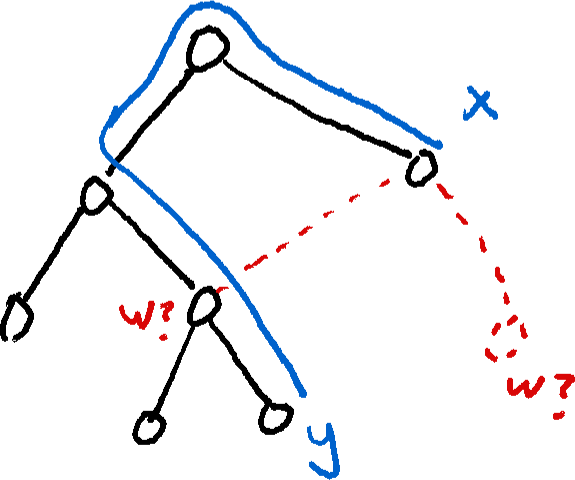
\includegraphics[width=0.5\textwidth]{graphics/L3_trees/lemma_trees_have_leaves.png}
      \caption[][0cm]{The two cases we consider in the proof of Lemma \ref{lemma:trees_have_leaves}, illustrated in dashed red lines, with the maximal path drawn in blue.}
      \label{fig:lemma_trees_have_leaves}
    \end{figure}

    Then $x$ has a neighbour $w$ different from $x_1$. There are two cases, which are also illustrated in Figure \ref{fig:lemma_trees_have_leaves}:
    \begin{enumerate}
      \item $w$ is not already a vertex on the path $P$. Then we could just extend the path to include $w$, contradicting our assumption that $P$ was maximal.
      \item $w$ is already a vertex on the path $P$. However, this must mean there is a cycle in the graph -- we can start walking along $T$ from $x$ until we reach $w$, and then loop back along the edge from $w$ to $x$ -- contradicting our assumption that the graph is a tree.
    \end{enumerate}

    So neither case is possible, and so we conclude that $d_x = d_y = 1$, proving the lemma.
  \end{proof}
\end{lemma}

We also get a very simple formula for the number of edges of a tree:

\begin{lemma}
  Any tree on $n$ vertices has $n-1$ edges.

  \begin{proof}
    We prove this by induction in the number of vertices. The base case is the simple graph on a single vertex, which clearly has one vertex and zero edges, satisfying the theorem.

    Now, suppose $T$ is a tree on $n > 1$ vertices. By Lemma \ref{lemma:trees_have_leaves}, it has at least two vertices of degree $1$. Pick one of them, say $x$, and remove it and the edge it is incident to from the graph.\sidenote[][]{So, formally, we are looking at the induced subgraph $T[V\setminus \{x\}]$.} 
    
    This leaves us with a tree on $n-1$ vertices, and so by our induction hypothesis it has $n-2$ edges. So by removing a vertex and an edge, we were left with $n-1$ vertices and $n-2$ edges -- so clearly we must have started with $n$ vertices and $n-1$ edges, as the lemma claimed.
  \end{proof}
\end{lemma}

We can actually give an exact count of the number of labelled trees on $n$ vertices as well. We will state the theorem here, but we postpone the proof of it until a later lecture, when we will have seen the Kirchhoff matrix-tree theorem, which is a nice way of proving it.\sidenote[][-1.8cm]{In previous years, this course included a proof of this theorem using Prüfer sequences. However, that proof -- and a different one using double counting -- is also included in the course on combinatorics in this department. So, in the interest of keeping the contents of the courses disjoint, we give the proof using the matrix-tree theorem instead.

If you are interested, and can read Swedish, you can find the other two proofs of this theorem in these lecture notes: \url{https://vagdur.github.io/Kombinatorik-1MA020/lecture8.pdf}.}

\begin{theorem}[Cayley's formula]
  There are $n^{n-2}$ labelled trees on $n$ vertices.
\end{theorem}

Having seen all these results about trees, let us give a result giving a few equivalent characterisations of trees:

\begin{theorem}\label{theorem:classification_of_trees}
  The following statements are equivalent:
  \begin{enumerate}
    \item $T$ is a tree.
    \item For any two vertices $x, y$ of $T$ there exists a unique path connecting $x$ and $y$.
    \item $T$ is edge-minimal among connected graphs, that is, removing any edge from it makes it disconnected.
    \item $T$ is edge-maximal among cycle-free graphs, that is, adding an edge between any two vertices introduces a cycle.
  \end{enumerate}

  \begin{proof}
    We will show that (1) implies (2), that (2) implies (3) and (4), and that both (3) and (4) imply (1), showing the theorem.

    $(1) \Rightarrow (2)$: Assume $T$ is a tree and $x$ and $y$ two vertices. Since $T$ is connected, there is at least one path from $x$ to $y$. If there was another distinct path, the union of the two paths would contain a cycle, which is impossible in a tree. Thus the path is unique.

    $(2) \Rightarrow (3)$: Consider any edge $\{x,y\} \in E$. By (2), this must in fact be the \emph{unique} path between $x$ and $y$, so removing this edge would disconnect these two vertices and thus the graph.

    $(2) \Rightarrow (4)$: Consider any two vertices $x, y \in T$. By (2), there is a unique path connecting them. Adding an edge $\{x,y\}$ would thus create a cycle -- walk along the path from $x$ to $y$ and then head back along the new edge.

    $(3) \Rightarrow (1)$: If $T$ is edge-minimal among connected graphs, it is of course connected. So what we need to show to show that it is a tree is that it contains no cycles. So, assume for contradiction that it has a cycle -- then we could delete an edge of this cycle without disconnecting the graph,\sidenote[][]{Why?} contradicting our assumption of edge-minimality.

    $(4) \Rightarrow (1):$ If $T$ is edge-maximal among cycle-free graphs, it is in particular cycle-free, and so what we need to show in order to show that it is a tree is that it is connected. So assume for contradiction that it is disconnected -- then we could add an edge between two connected components without introducing any cycles, contradicing our assumption of edge-maximality.
  \end{proof}
\end{theorem}

\section{Spanning trees}

Recall from last lecture that a subgraph is said to be spanning if it contains all vertices of $G$. This notion is particularly interesting if the subgraph is a tree.

\begin{figure}
  \centering
  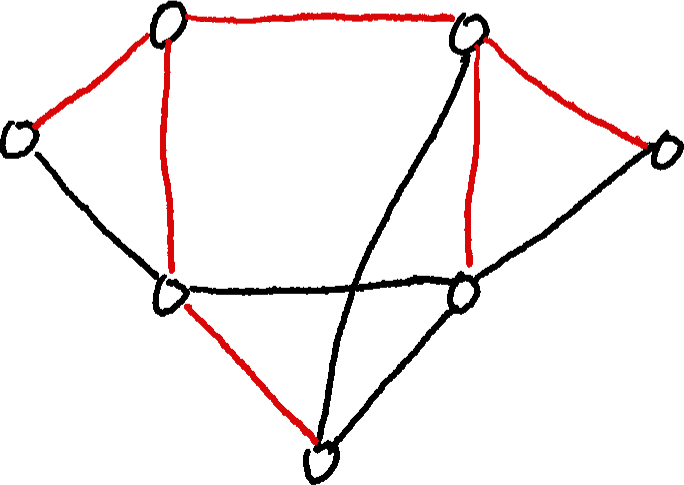
\includegraphics[width=0.5\textwidth]{graphics/L3_trees/spanning_tree.png}
  \caption[][0cm]{A graph $G$, with a spanning tree highlighted in red.}
  \label{fig:spanning_tree}
\end{figure}

\begin{definition}
  Let $G$ be a graph, simple or multi. A \emph{spanning tree} of $G$ is a spanning subgraph that is a tree. One example is given in Figure \ref{fig:spanning_tree}.
\end{definition}

Obviously, a graph that is disconnected cannot have any spanning trees -- and for finite graphs, this condition is also sufficient.\sidenote[][-0.8cm]{
  \begin{xca}
    Give a proof of this that does not rely on the axiom of choice.
  \end{xca}
} For infinite graphs, the situation is somewhat hairier -- the statement that \emph{all} graphs have spanning trees is in fact equivalent to the axiom of choice!

Before proving this statement under the assumption of choice, let us state the form of the axiom of choice that we will be using.

\begin{lemma}[Zorn's lemma]
  Let $(A, \leq)$ be a non-empty partially ordered set. A subset $C \subseteq A$ is a \emph{chain} if for any two elements $c, c' \in C$, we either have $c \leq c'$ or $c' \leq c$. Assume that for every chain $C$ in $A$ there exists an upper bound $b \in A$, that is, an element such that $c \leq b$ for all $c \in C$. Then there exists a maximal element $m$ of $A$, that is, an $m$ such that $m \not\leq a$ for any $a \neq m$.
\end{lemma}

Having stated this, we can now proceed to state and prove our theorem about spanning trees.

\begin{theorem}
  Assuming the axiom of choice, all (multi)graphs have a spanning tree.

  \begin{proof}
    Let $G = (V,E)$ be some graph. We will apply Zorn's lemma with $A$ as the set of all cycle-free spanning subgraphs of $G$, and $\leq$ as the ``is a subgraph of'' relation.\sidenote[][]{Here we mean literal subgraph of, not just ``isomorphic to a subgraph of'' -- we really need one to be a subset of the other.} This gives $A$ the structure of a partially ordered set -- and it is nonempty since the subgraph containing all the vertices and none of the edges is trivially spanning and cycle free.

    So, let $C$ be some chain in $A$, consisting of elements $H_i = (V, E_i)$ for $i \in I$,\sidenote[][]{We really need the index \emph{set} $I$ here, not just integer indices -- the cardinality of $C$ could be enormous!} and define
    $$B = \left(V, \bigcup_{i\in I} E_i\right).$$
    We want to show that $B$ is an upper bound for the chain $C$ -- if we can do this, Zorn's lemma will apply and give us the theorem.

    By construction, $B$ is a spanning subgraph of $G$. We want to show that it is an element of $A$, so we need to show that it is also cycle-free. So, assume for contradiction that it contains some cycle consisting of edges $e_1, e_2, \ldots, e_r$. Each of these edges must then be contained in some $H_i$ -- let us say that $e_j$ is contained in $H_{i(j)}$.

    Since $C$ is a chain, one of these graphs $H_{i(1)}, H_{i(2)}, \ldots, H_{i(r)}$ must contain all of the others -- say it is $H_j$. Then this $H_j$ must contain all of the edges $e_1, e_2, \ldots, e_r$, and so contain a cycle -- but this is a contradiction, since $H_j$ is an element of $A$ and thus cycle-free.

    Now, we need to show that $B$ is indeed an upper bound of the chain $C$, in order for Zorn's lemma to apply. This, however, is easy -- of course $E_i \subseteq \bigcup_{i\in I} E_i$, and so $H_i$ is a subgraph of $B$ for each $i$.

    The conclusion of Zorn's lemma now gives us the existence of a cycle-free spanning subgraph that is maximal with respect to the subgraph ordering, which in this case means it is edge-maximal. So, by an analogous argument as in Theorem \ref{theorem:classification_of_trees},\sidenote[][]{We can't quite apply this theorem directly, because it assumes it is edge-maximal among \emph{all} cycle-free graphs, not just among the cycle-free subgraphs of a fixed graph. In last year's lecture notes they just appeal to this theorem, but that seems to me to be subtly wrong.} this maximal subgraph is in fact a tree, and so we have found our desired spanning tree.
  \end{proof}
\end{theorem}

\begin{theorem}
  
\end{theorem}

\section{Exercises}

\begin{xca}
  We proved that all graphs, including infinite graphs, have a spanning tree using the axiom of choice in the lecture, and we stated that in fact the two are equivalent.

  Prove the axiom of choice using the assumption that all graphs have spanning trees.
\end{xca}
%\bibliography{references}
%\bibliographystyle{plainnat}

\end{document}
